\documentclass[12pt]{IEEEtran}
\usepackage[utf8]{inputenc}
\usepackage{graphicx}
\usepackage{amsmath, amsthm, amssymb}

\title{Chaos Project 1}
\author{
  Paul Booth \\
  \and
  Geoff Pleiss
}
\date{}

\newtheorem{thm}{Theorem}
\newtheorem{lma}{Lemma}

\begin{document}
  \maketitle

\begin{abstract}
\end{abstract}



\section{Introduction}
The theorem we are trying to prove is

\begin{thm}
\label{thm:mainthm}
	Let $J$ be an interval and let $F$ be a continuous first-order map with $F : J \rightarrow J$. If there is some point $a \in J$ that satisfies the following
	%
	\[ F^3\left(a\right) \leq a < F\left(a\right) < F^2\left(a\right) \]
	or
	\[ F^3\left(a\right) \geq a > F\left(a\right) > F^2\left(a\right) \]
	%
	then $J$ contains a $k$-period orbit for all $k \in \mathbb{N}$.
\end{thm}

In the first section we will provide a rough outline of the proof for this theorem, which will be followed by the proof in full. We will then discuss the interpretations and implications of our results.



\section{The big picture}

In order to prove that a first-order map $F$ contains an orbit with period $k$, there are two things we must prove. First, we must show that there is a fixed point on the $k^{th}$ return map of F. In other words, we must show that there is some $x \in J$ for which $F^k \left( x \right) = x$. To understand why this implies periodicity, let's examine $F^2k \left( x \right)$. This is simply equal to $F^k \left( F^k \left( x \right) \right) = F^k \left( x \right) = x$. A simple inductive proof will show that $F^n \left( x \right) = x$ whenever $n \equiv 0 \left(\mod k \right)$, thus showing that $x$ is a periodic point.

However, even if we find a fixed point $x$ of $F^k$, this does not imply that the periodicity of $x$ is $k$. For example, $x$ could also be a fixed point of $F^{k/2}$. Thus $2$ orbits of $F$ would be completed $k$ iterations of the function, and so the periodicity of $x$ would be $k/2$. To show that $x$ has periodicity of $k$, we must also show that $x$ is {\it not} a fixed point of $F^m$ for any $m < k$.

If we show that there is some $x \in J$ that meets these criteria for an arbitrary $k$, then we will have proven that $F$ has orbits of every periodicity.



\section{Lemmas}
% TODO: FIGURE OUT HOW WE WANT TO PRESENT THIS ACTUALLY

\begin{lma}
\label{lma:cont_comp}
	Continuity / compactness
\end{lma}

\begin{figure}
\label{fig:continuity_graph}
	\begin{center}
		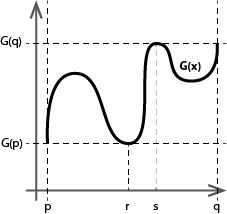
\includegraphics{img/continuity_graph.png}
		\caption{Diagram for Lemma \ref{lma:cont_comp}}
	\end{center}
\end{figure}



\section{Implications/Conclusions}

Though it appears that we have shown that there is some arbitrary number of fixed points of $F^k$, we can actually say a bit more about how many fixed points exist. Let $x_0$ be a point with periodicity of exactly $k$ for the function $F$. 

Define $x_1$, $x_2$, $\cdots$, $x_{k-1}$ to be $F \left( x_0 \right)$, $F^2 \left( x_0 \right)$, $\cdots$, $F^{k-1} \left( x_0 \right)$, respectively. We know that $x_1$ cannot equal $x_0$ because otherwise the periodicity of $x$ would be less than $k$. We also know that $x_1$  cannot equal $x_2$, $x_3$, \cdots $x_{k-1}$. Assume that there was some $l < k-1$ where $x_1 = x_l$. Then the sequence $x_n = F^n \left( x \right)$ would have terms $x_0$, $x_1$, $x_2$, $\cdots$, $x_l = x_1$, $x_2$, $\cdots$. Note that this sequence never returns to $x_0$, which would make $x_0$ a non-periodic point. Thus $x_1$ is a unique point, and it does not have periodicity less than $k$. A similar argument can be made for all the other points.

Now we can show that our $k$ points -- $x_0$, $x_1$, $\cdots$, $x_{k-1}$ -- are $k$-periodic. Given $x_l$, we know that $F^k \left( x_l \right) = F^{k+l} \left ( x_0 \right) = F^{l} \left ( x_0 \right) = x_l$. Thus we have shown that for each $l \in [0,k-1]$, $x_l$ is a unique point with periodicity of exactly $k$. Thus there are at least $k$ points that are $k$-periodic on the map $F$. If there was a $k+1^{th}$ unique $k$-periodic point, we could use a similar argument to show that there must be an additional $k-1$ more $k$-periodic points that lie on the $k+1^{th}$ point's orbit. To summarize, on any given map $F$ for which Theorem \ref{thm:main_theorem} applies, there are exatly $n \left( k \right)$ points with periodicity $k$, where $n \in \mathbb{N}$.



\end{document}

